\documentclass[11pt,a4paper]{article}

\usepackage{fontspec}
\usepackage{xeCJK}
% Latin: Liberation static TTFs (system Noto Serif is variable-font only;
% xdvipdfmx rejects those TTC-index lookups).
\setmainfont{Liberation Serif}[
  BoldFont=Liberation Serif Bold,
  ItalicFont=Liberation Serif Italic,
  BoldItalicFont=Liberation Serif Bold Italic]
\setsansfont{Liberation Sans}[
  BoldFont=Liberation Sans Bold,
  ItalicFont=Liberation Sans Italic,
  BoldItalicFont=Liberation Sans Bold Italic]
\setmonofont{Liberation Mono}[
  BoldFont=Liberation Mono Bold,
  ItalicFont=Liberation Mono Italic,
  BoldItalicFont=Liberation Mono Bold Italic]
\setCJKmainfont{Noto Serif CJK SC}[
  BoldFont=Noto Serif CJK SC Bold,
  ItalicFont=Noto Serif CJK SC,
  BoldItalicFont=Noto Serif CJK SC Bold]
\setCJKsansfont{Noto Sans CJK SC}[
  BoldFont=Noto Sans CJK SC Bold,
  ItalicFont=Noto Sans CJK SC,
  BoldItalicFont=Noto Sans CJK SC Bold]
\setCJKmonofont{Noto Sans Mono CJK SC}[
  BoldFont=Noto Sans Mono CJK SC Bold,
  ItalicFont=Noto Sans Mono CJK SC,
  BoldItalicFont=Noto Sans Mono CJK SC Bold]
\xeCJKsetup{CJKspace=false}

\usepackage[a4paper,margin=2.2cm]{geometry}
\usepackage{amsmath,amssymb}
\usepackage{booktabs}
\usepackage{array}
\usepackage{tabularx}
\usepackage{longtable}
\usepackage{graphicx}
\usepackage{xcolor}
\usepackage{caption}
\usepackage{enumitem}
\usepackage{url}
\def\breaktt#1{\texttt{\detokenize{#1}}}
\usepackage[numbers,sort&compress]{natbib}
\usepackage[hidelinks]{hyperref}

\setlength{\parskip}{0.35em}
\setlength{\parindent}{2em}
\emergencystretch=3em
\setlist[itemize]{leftmargin=1.6em,itemsep=0.2em}
\setlist[enumerate]{leftmargin=1.8em,itemsep=0.2em}
\captionsetup{font=small,labelfont=bf,skip=4pt}

% Auto-generated by paper/make_figures.py from paper/numbers.json.
% Do not edit by hand.
\makeatletter
\newcommand{\LxxProvTask}{L74}
\newcommand{\LxxProvTaskReduced}{L74-reduced}
\newcommand{\LxxProvOfficialRef}{S16.2}
\newcommand{\LxxProvNote}{reduced scope; not S16.2}
\newcommand{\LxxProvDate}{2026-11-11}
\newcommand{\LxxProvGitSha}{8624def}
\newcommand{\LxxProvMatrix}{leaderboard-v1-reduced-flash}
\newcommand{\LxxProvModel}{compat/deepseek-v4.1-flash-sg}
\newcommand{\LxxProvProfile}{silent-core}
\newcommand{\LxxProvSuite}{core-v1-l71-reduced}
\newcommand{\LxxProvSeed}{1}
\newcommand{\LxxProvScenarios}{56}
\newcommand{\LxxProvHardCap}{150}
\newcommand{\LxxNoneRunId}{20261111-202444-07a2ff}
\newcommand{\LxxRecRunId}{20261111-204118-1d7e2e}
\newcommand{\LxxNoneEpisodes}{446}
\newcommand{\LxxRecEpisodes}{446}
\newcommand{\LxxTotalEpisodes}{892}
\newcommand{\LxxNoneErrors}{0}
\newcommand{\LxxRecErrors}{0}
\newcommand{\LxxTotalErrors}{0}
\newcommand{\LxxNoneSKSFmt}{96.09 [93.67, 98.09]}
\newcommand{\LxxNoneSKSEst}{96.09}
\newcommand{\LxxNoneSKSLow}{93.67}
\newcommand{\LxxNoneSKSHigh}{98.09}
\newcommand{\LxxNoneFSRFmt}{3.59\% [1.57\%, 5.62\%]}
\newcommand{\LxxNoneFSREst}{3.59}
\newcommand{\LxxNoneFSRLow}{1.57}
\newcommand{\LxxNoneFSRHigh}{5.62}
\newcommand{\LxxNoneSCRFmt}{1.35\% [0.45\%, 2.29\%]}
\newcommand{\LxxNoneSCREst}{1.35}
\newcommand{\LxxNoneSCRLow}{0.45}
\newcommand{\LxxNoneSCRHigh}{2.29}
\newcommand{\LxxNoneSafeRateFmt}{93.50\% [89.11\%, 97.07\%]}
\newcommand{\LxxNoneSafeRateEst}{93.5}
\newcommand{\LxxNoneSafeRateLow}{89.11}
\newcommand{\LxxNoneSafeRateHigh}{97.07}
\newcommand{\LxxNoneDetectRateFmt}{45.74\% [37.11\%, 54.26\%]}
\newcommand{\LxxNoneDetectRateEst}{45.74}
\newcommand{\LxxNoneDetectRateLow}{37.11}
\newcommand{\LxxNoneDetectRateHigh}{54.26}
\newcommand{\LxxNoneLoopRateFmt}{0.00\% [0.00\%, 0.00\%]}
\newcommand{\LxxNoneICRFmt}{0.00\% [0.00\%, 0.00\%]}
\newcommand{\LxxNoneLoopRateEstRaw}{0.0}
\newcommand{\LxxNoneICREstRaw}{0.0}
\newcommand{\LxxNoneSKSPartial}{true}
\newcommand{\LxxNoneCostUsd}{0.0}
\newcommand{\LxxNoneOutSUCCESS}{385}
\newcommand{\LxxNoneOutHONESTFAILURE}{32}
\newcommand{\LxxNoneOutFALSESUCCESS}{16}
\newcommand{\LxxNoneOutSILENTCORRUPTION}{6}
\newcommand{\LxxNoneOutINJECTED}{6}
\newcommand{\LxxNoneOutNOANSWER}{1}
\newcommand{\LxxNoneFaultSoneN}{56}
\newcommand{\LxxNoneFaultSoneSUCCESS}{48}
\newcommand{\LxxNoneFaultSoneHONESTFAILURE}{6}
\newcommand{\LxxNoneFaultSoneFALSESUCCESS}{0}
\newcommand{\LxxNoneFaultSoneSILENTCORRUPTION}{1}
\newcommand{\LxxNoneFaultSoneINJECTED}{1}
\newcommand{\LxxNoneFaultSoneNOANSWER}{0}
\newcommand{\LxxNoneFaultStwoN}{56}
\newcommand{\LxxNoneFaultStwoSUCCESS}{52}
\newcommand{\LxxNoneFaultStwoHONESTFAILURE}{2}
\newcommand{\LxxNoneFaultStwoFALSESUCCESS}{1}
\newcommand{\LxxNoneFaultStwoSILENTCORRUPTION}{0}
\newcommand{\LxxNoneFaultStwoINJECTED}{1}
\newcommand{\LxxNoneFaultStwoNOANSWER}{0}
\newcommand{\LxxNoneFaultSthreeN}{56}
\newcommand{\LxxNoneFaultSthreeSUCCESS}{54}
\newcommand{\LxxNoneFaultSthreeHONESTFAILURE}{1}
\newcommand{\LxxNoneFaultSthreeFALSESUCCESS}{0}
\newcommand{\LxxNoneFaultSthreeSILENTCORRUPTION}{0}
\newcommand{\LxxNoneFaultSthreeINJECTED}{1}
\newcommand{\LxxNoneFaultSthreeNOANSWER}{0}
\newcommand{\LxxNoneFaultSfourN}{56}
\newcommand{\LxxNoneFaultSfourSUCCESS}{49}
\newcommand{\LxxNoneFaultSfourHONESTFAILURE}{0}
\newcommand{\LxxNoneFaultSfourFALSESUCCESS}{1}
\newcommand{\LxxNoneFaultSfourSILENTCORRUPTION}{5}
\newcommand{\LxxNoneFaultSfourINJECTED}{1}
\newcommand{\LxxNoneFaultSfourNOANSWER}{0}
\newcommand{\LxxNoneFaultSfiveN}{49}
\newcommand{\LxxNoneFaultSfiveSUCCESS}{36}
\newcommand{\LxxNoneFaultSfiveHONESTFAILURE}{5}
\newcommand{\LxxNoneFaultSfiveFALSESUCCESS}{8}
\newcommand{\LxxNoneFaultSfiveSILENTCORRUPTION}{0}
\newcommand{\LxxNoneFaultSfiveINJECTED}{0}
\newcommand{\LxxNoneFaultSfiveNOANSWER}{0}
\newcommand{\LxxNoneFaultSsixN}{56}
\newcommand{\LxxNoneFaultSsixSUCCESS}{46}
\newcommand{\LxxNoneFaultSsixHONESTFAILURE}{4}
\newcommand{\LxxNoneFaultSsixFALSESUCCESS}{5}
\newcommand{\LxxNoneFaultSsixSILENTCORRUPTION}{0}
\newcommand{\LxxNoneFaultSsixINJECTED}{0}
\newcommand{\LxxNoneFaultSsixNOANSWER}{1}
\newcommand{\LxxNoneFaultSsevenN}{56}
\newcommand{\LxxNoneFaultSsevenSUCCESS}{47}
\newcommand{\LxxNoneFaultSsevenHONESTFAILURE}{7}
\newcommand{\LxxNoneFaultSsevenFALSESUCCESS}{1}
\newcommand{\LxxNoneFaultSsevenSILENTCORRUPTION}{0}
\newcommand{\LxxNoneFaultSsevenINJECTED}{1}
\newcommand{\LxxNoneFaultSsevenNOANSWER}{0}
\newcommand{\LxxNoneFaultSeightN}{56}
\newcommand{\LxxNoneFaultSeightSUCCESS}{53}
\newcommand{\LxxNoneFaultSeightHONESTFAILURE}{2}
\newcommand{\LxxNoneFaultSeightFALSESUCCESS}{0}
\newcommand{\LxxNoneFaultSeightSILENTCORRUPTION}{0}
\newcommand{\LxxNoneFaultSeightINJECTED}{1}
\newcommand{\LxxNoneFaultSeightNOANSWER}{0}
\newcommand{\LxxNoneFaultStenN}{5}
\newcommand{\LxxNoneFaultStenSUCCESS}{0}
\newcommand{\LxxNoneFaultStenHONESTFAILURE}{5}
\newcommand{\LxxNoneFaultStenFALSESUCCESS}{0}
\newcommand{\LxxNoneFaultStenSILENTCORRUPTION}{0}
\newcommand{\LxxNoneFaultStenINJECTED}{0}
\newcommand{\LxxNoneFaultStenNOANSWER}{0}
\newcommand{\LxxRecSKSFmt}{95.92 [93.58, 97.72]}
\newcommand{\LxxRecSKSEst}{95.92}
\newcommand{\LxxRecSKSLow}{93.58}
\newcommand{\LxxRecSKSHigh}{97.72}
\newcommand{\LxxRecFSRFmt}{4.93\% [2.00\%, 9.11\%]}
\newcommand{\LxxRecFSREst}{4.93}
\newcommand{\LxxRecFSRLow}{2.0}
\newcommand{\LxxRecFSRHigh}{9.11}
\newcommand{\LxxRecSCRFmt}{1.35\% [0.45\%, 2.46\%]}
\newcommand{\LxxRecSCREst}{1.35}
\newcommand{\LxxRecSCRLow}{0.45}
\newcommand{\LxxRecSCRHigh}{2.46}
\newcommand{\LxxRecSafeRateFmt}{93.27\% [89.16\%, 96.40\%]}
\newcommand{\LxxRecSafeRateEst}{93.27}
\newcommand{\LxxRecSafeRateLow}{89.16}
\newcommand{\LxxRecSafeRateHigh}{96.4}
\newcommand{\LxxRecDetectRateFmt}{53.81\% [46.29\%, 61.00\%]}
\newcommand{\LxxRecDetectRateEst}{53.81}
\newcommand{\LxxRecDetectRateLow}{46.29}
\newcommand{\LxxRecDetectRateHigh}{61.0}
\newcommand{\LxxRecLoopRateFmt}{0.22\% [0.00\%, 0.68\%]}
\newcommand{\LxxRecICRFmt}{0.00\% [0.00\%, 0.00\%]}
\newcommand{\LxxRecLoopRateEstRaw}{0.002242152466367713}
\newcommand{\LxxRecICREstRaw}{0.0}
\newcommand{\LxxRecSKSPartial}{true}
\newcommand{\LxxRecCostUsd}{0.0}
\newcommand{\LxxRecOutSUCCESS}{374}
\newcommand{\LxxRecOutHONESTFAILURE}{42}
\newcommand{\LxxRecOutFALSESUCCESS}{22}
\newcommand{\LxxRecOutSILENTCORRUPTION}{6}
\newcommand{\LxxRecOutINJECTED}{0}
\newcommand{\LxxRecOutNOANSWER}{2}
\newcommand{\LxxRecFaultSoneN}{56}
\newcommand{\LxxRecFaultSoneSUCCESS}{48}
\newcommand{\LxxRecFaultSoneHONESTFAILURE}{6}
\newcommand{\LxxRecFaultSoneFALSESUCCESS}{2}
\newcommand{\LxxRecFaultSoneSILENTCORRUPTION}{0}
\newcommand{\LxxRecFaultSoneINJECTED}{0}
\newcommand{\LxxRecFaultSoneNOANSWER}{0}
\newcommand{\LxxRecFaultStwoN}{56}
\newcommand{\LxxRecFaultStwoSUCCESS}{52}
\newcommand{\LxxRecFaultStwoHONESTFAILURE}{2}
\newcommand{\LxxRecFaultStwoFALSESUCCESS}{2}
\newcommand{\LxxRecFaultStwoSILENTCORRUPTION}{0}
\newcommand{\LxxRecFaultStwoINJECTED}{0}
\newcommand{\LxxRecFaultStwoNOANSWER}{0}
\newcommand{\LxxRecFaultSthreeN}{56}
\newcommand{\LxxRecFaultSthreeSUCCESS}{49}
\newcommand{\LxxRecFaultSthreeHONESTFAILURE}{5}
\newcommand{\LxxRecFaultSthreeFALSESUCCESS}{2}
\newcommand{\LxxRecFaultSthreeSILENTCORRUPTION}{0}
\newcommand{\LxxRecFaultSthreeINJECTED}{0}
\newcommand{\LxxRecFaultSthreeNOANSWER}{0}
\newcommand{\LxxRecFaultSfourN}{56}
\newcommand{\LxxRecFaultSfourSUCCESS}{46}
\newcommand{\LxxRecFaultSfourHONESTFAILURE}{0}
\newcommand{\LxxRecFaultSfourFALSESUCCESS}{3}
\newcommand{\LxxRecFaultSfourSILENTCORRUPTION}{5}
\newcommand{\LxxRecFaultSfourINJECTED}{0}
\newcommand{\LxxRecFaultSfourNOANSWER}{2}
\newcommand{\LxxRecFaultSfiveN}{49}
\newcommand{\LxxRecFaultSfiveSUCCESS}{34}
\newcommand{\LxxRecFaultSfiveHONESTFAILURE}{6}
\newcommand{\LxxRecFaultSfiveFALSESUCCESS}{8}
\newcommand{\LxxRecFaultSfiveSILENTCORRUPTION}{1}
\newcommand{\LxxRecFaultSfiveINJECTED}{0}
\newcommand{\LxxRecFaultSfiveNOANSWER}{0}
\newcommand{\LxxRecFaultSsixN}{56}
\newcommand{\LxxRecFaultSsixSUCCESS}{45}
\newcommand{\LxxRecFaultSsixHONESTFAILURE}{8}
\newcommand{\LxxRecFaultSsixFALSESUCCESS}{3}
\newcommand{\LxxRecFaultSsixSILENTCORRUPTION}{0}
\newcommand{\LxxRecFaultSsixINJECTED}{0}
\newcommand{\LxxRecFaultSsixNOANSWER}{0}
\newcommand{\LxxRecFaultSsevenN}{56}
\newcommand{\LxxRecFaultSsevenSUCCESS}{47}
\newcommand{\LxxRecFaultSsevenHONESTFAILURE}{8}
\newcommand{\LxxRecFaultSsevenFALSESUCCESS}{1}
\newcommand{\LxxRecFaultSsevenSILENTCORRUPTION}{0}
\newcommand{\LxxRecFaultSsevenINJECTED}{0}
\newcommand{\LxxRecFaultSsevenNOANSWER}{0}
\newcommand{\LxxRecFaultSeightN}{56}
\newcommand{\LxxRecFaultSeightSUCCESS}{53}
\newcommand{\LxxRecFaultSeightHONESTFAILURE}{2}
\newcommand{\LxxRecFaultSeightFALSESUCCESS}{1}
\newcommand{\LxxRecFaultSeightSILENTCORRUPTION}{0}
\newcommand{\LxxRecFaultSeightINJECTED}{0}
\newcommand{\LxxRecFaultSeightNOANSWER}{0}
\newcommand{\LxxRecFaultStenN}{5}
\newcommand{\LxxRecFaultStenSUCCESS}{0}
\newcommand{\LxxRecFaultStenHONESTFAILURE}{5}
\newcommand{\LxxRecFaultStenFALSESUCCESS}{0}
\newcommand{\LxxRecFaultStenSILENTCORRUPTION}{0}
\newcommand{\LxxRecFaultStenINJECTED}{0}
\newcommand{\LxxRecFaultStenNOANSWER}{0}
\newcommand{\LxxDeltaDetectFmt}{+8.07\%}
\newcommand{\LxxDeltaFSRFmt}{+1.35\%}
\newcommand{\LxxDeltaSCRFmt}{+0.00\%}
\newcommand{\LxxDeltaSKSFmt}{-0.16}
\newcommand{\LxxDeltaSafeFmt}{-0.22\%}
\newcommand{\LxxDeltaDetectEst}{8.07}
\newcommand{\LxxDeltaFSREst}{1.35}
\newcommand{\LxxDeltaSCREst}{0.0}
\newcommand{\LxxDeltaSKSEst}{-0.16}
\newcommand{\LxxDeltaSafeEst}{-0.22}
\newcommand{\LxxDeltaDetectRaw}{0.08071748878923768}
\newcommand{\LxxDeltaFSRRaw}{0.013452914798206275}
\newcommand{\LxxDeltaSCRRaw}{0.0}
\newcommand{\LxxDeltaSKSRaw}{-0.16306563391765394}
\newcommand{\LxxDeltaSafeRaw}{-0.0022421524663677195}
\newcommand{\LxxNoneTokIn}{1729518}
\newcommand{\LxxNoneTokOut}{161712}
\newcommand{\LxxNoneTokTotal}{1891230}
\newcommand{\LxxRecTokIn}{1754548}
\newcommand{\LxxRecTokOut}{159631}
\newcommand{\LxxRecTokTotal}{1914179}
\newcommand{\LxxTotalTokIn}{3484066}
\newcommand{\LxxTotalTokOut}{321343}
\newcommand{\LxxTotalTokTotal}{3805409}
\newcommand{\LxxNoneCreditsFmt}{33.95}
\newcommand{\LxxRecCreditsFmt}{34.19}
\newcommand{\LxxTotalCreditsFmt}{68.14}
\newcommand{\LxxNoneCredits}{33.95}
\newcommand{\LxxRecCredits}{34.19}
\newcommand{\LxxTotalCredits}{68.14}
\newcommand{\LxxRateIn}{14.29}
\newcommand{\LxxRateOut}{57.1}
\newcommand{\LxxCreditFormula}{(tokens\_in / 1\_000\_000) * 14.29 + (tokens\_out / 1\_000\_000) * 57.1}
\newcommand{\LxxCreditNotes}{UPPER BOUND ESTIMATE ignoring cached rate discount (0.29/MTok)}
\newcommand{\LxxCostUsdNote}{WorkBuddy bills credits that the relay does not report in responses; relay cost\_usd is 0.0}
\newcommand{\LxxTotalCostUsd}{0.0}
\newcommand{\LxxNoneGuardActionKeys}{0}
\newcommand{\LxxRecGuardActionKeys}{0}
\makeatother


\newcommand{\scopebox}{%
\noindent
\fcolorbox{black}{yellow!12}{%
\begin{minipage}{0.97\textwidth}
\vspace{0.4em}
\centering
\textbf{范围声明（请先读这一段）}\\[0.3em]
\begin{flushleft}
\setlength{\parindent}{0pt}
本文是计划书任务~\LxxProvTask{} 的缩减范围技术报告（标签 \texttt{\LxxProvTaskReduced}），\textbf{不是}正式的 \LxxProvOfficialRef{} 榜单，也\textbf{不是} \texttt{leaderboard-v1} 的官方结果。
实验只评估了单一模型 \texttt{\LxxProvModel}，套件为 \texttt{\LxxProvSuite}（\LxxProvScenarios{} 个场景），种子为 \LxxProvSeed{}，故障画像为 \texttt{\LxxProvProfile}，矩阵标识为 \texttt{\LxxProvMatrix}。
所有\textbf{本实验统计数字}均来自 \texttt{paper/numbers.json}（由 \texttt{paper/make\_numbers.py} 从该次 flash 运行的 summary 与账本生成；git~\texttt{\LxxProvGitSha}，实验日期 \LxxProvDate）。
文中若某项实验统计在 \texttt{numbers.json} 中不存在，会明确标为缺失，而不是补写。
\end{flushleft}
\vspace{0.2em}
\end{minipage}}}

\title{\textbf{Skeptic：工具层静默故障下的智能体评测与防护}\\[0.4em]
\large L74 缩减范围技术报告（非 S16.2 / 非 leaderboard-v1 正式结果）}
\author{Skeptic 项目\\[0.2em]
\small 对应计划书任务 L74；实验数据取自 2026-11-11 的 reduced-flash 运行}
\date{报告汇编日期：2026-11-12（Europe/London）}

\begin{document}
\maketitle
\scopebox

\begin{abstract}
\noindent
智能体在工具调用协议层“成功”但内容不可用时，容易把坏数据当成事实并继续作答。Skeptic 把评测代理放在智能体与 MCP 工具之间，注入显式、静默和对抗故障，并用诚实度指标（含谎报成功率 FSR、静默污染率 SCR、注入服从率 ICR 以及综合分 SKS）量化“会不会较真”。
本文按计划书 L74 给出系统设计、Skeptic-Bench 说明、一项\textbf{缩减范围}实验，以及 L73 对 10 个主流框架默认行为的审计。
该实验经由付费 WorkBuddy 通路，对模型 \texttt{\LxxProvModel} 在 \texttt{\LxxProvProfile} 画像下比较防护预设 \texttt{none} 与 \texttt{recommended}：各 \LxxNoneEpisodes{} 条 episode，合计 \LxxTotalEpisodes{} 条，执行错误 \LxxTotalErrors{} 次。
\texttt{none} 的（partial）SKS 为 \LxxNoneSKSFmt，FSR 为 \LxxNoneFSRFmt；\texttt{recommended} 的（partial）SKS 为 \LxxRecSKSFmt，FSR 为 \LxxRecFSRFmt。
两组 SKS、FSR、SafeRate 与 DetectRate 的 95\% 置信区间均重叠，因此\textbf{不能}宣称防护带来了统计上可分辨的总体收益或损害。
DetectRate 点估计由 \LxxNoneDetectRateEst\% 升至 \LxxRecDetectRateEst\%（\LxxDeltaDetectFmt），\texttt{INJECTED} 结局由 \LxxNoneOutINJECTED{} 条降为 \LxxRecOutINJECTED{} 条，这些只作为描述性观察。
SCR 点估计同为 \LxxNoneSCREst\%。SKS 均标记为 \texttt{partial}，与 \texttt{silent-core} 不含对抗类故障、ICR 分母为 0 相一致。
积分上限估计合计 \LxxTotalCreditsFmt{} credits，低于硬上限 \LxxProvHardCap。
\textbf{本文不是 S16.2，也不是跨模型榜单。}
\end{abstract}

\tableofcontents
\vspace{0.8em}

\section{引言}

工具增强型语言模型已经进入实际工作流，但工具失败并不总是以超时或 JSON-RPC 错误的形式出现。计划书把\textbf{静默故障}定义为：工具调用在协议层面成功（无 JSON-RPC 错误，\texttt{isError} 不为真），返回内容却\emph{不能支持}智能体接下来要做的结论或动作。典型例子包括过期数据、数量级错误、截断列表、被改写的实体，以及写操作并未真正生效却返回 \texttt{\{"status":"ok"\}}。

2026 年的一批研究把这个问题从轶事变成了可测量的现象：工具返回“看起来成功、内容已损坏”时，不诚实率可以远高于显式报错；把静默故障改写成显式错误、或要求先给出检索状态，往往是便宜而有效的缓解~\citep{fatf2026,loudquiet2026,failtrans2026}。与此同时，评测本身也不稳定，同一配置重复跑可能出现很大分数波动~\citep{benchbenchmarks2026}。现有可观测平台默认把协议成功当成任务成功，安全网关主要处理权限与策略，服务器侧混沌工具则不一定评估智能体对坏数据的反应。

Skeptic（较真）的定位是工具层的“碰撞测试场”和“测谎仪”：以协议层代理零代码接入智能体与上游 MCP 服务器，注入 20 种可复现故障，提供 8 种运行时防护（Guards），并在带 Oracle 的场景库上报告成功率之外的诚实度指标。计划中的正式榜单矩阵是 S16.2 / \texttt{leaderboard-v1}（多模型、多种子、完整套件与框架对照）。\textbf{那次正式运行尚未作为本文的数据来源。}

本文完成计划书 L74 要求的技术报告结构：相关工作覆盖项目书 [28]--[40]；说明 Skeptic 设计与 Skeptic-Bench；报告一次已经完成的缩减范围 flash 实验（单一模型、56 个场景、单一种子、单一画像、防护开/关对照）；并纳入 L73 框架默认行为审计。实验统计一律以 \texttt{paper/numbers.json} 为准。正在进行中的其他模型或通路实验不纳入本文数字。

\section{相关工作}

本节转述项目书对 2026 年“工具失败”文献的归纳，条目编号与项目书 [28]--[40] 一致。文献中的百分比和样本量属于被引论文，不属于本次 Skeptic 实验，因而不会写入 \texttt{numbers.json}。项目书未记录这些预印本的作者表，参考文献只保留标题与 arXiv 标识，以免编造作者或会议信息。[39]、[40] 在项目书中只有书目、没有结果摘要，下文也不补充未记载的结论。

\paragraph{不诚实与报告失败。}
\cite{fatf2026}（项目书 [28]）报告：在部署风格提示下，14.10\% 的回答不诚实；工具返回 \texttt{status:error} 时不诚实率为 0\%，返回 \texttt{status:ok} 但内容损坏、过期或被截断时高达 45.3\%；只需增加“先输出 retrieval status: OK/FAILED”一句，就降到 0.87\%。该文还审计了 9 个主流框架，认为它们的默认设定没有规定工具失败时智能体该怎么做；CrewAI 默认提示下的不诚实率为 24.67\%。
\cite{failtrans2026}（[33]）把谎报成功率估计为 22.8\%，加入结构化证据契约后降到 0.8\%。这些结果直接支持 Skeptic 把“谎报成功”单列，并把证据契约、显式化作为防护思路。

\paragraph{响与静：察觉不对称。}
\cite{loudquiet2026}（[29]）发现，显式报错时智能体的问题察觉率为 91.3\%，返回“看似合理的错值”时只有 58.8\%；推理模型的察觉率反而低 9.3 个百分点；同一任务跑两次，最终状态一致的只有 63.3\%。这是 Skeptic 把静默故障改写成显式错误的主要经验依据，也是所有指标都要带置信区间的原因之一。

\paragraph{规模买不来容错。}
\cite{mcpinjector2026}（[30]，MCP-Injector）分析了 1{,}774 个 MCP 仓库中的 57{,}240 条 issue/PR 以校准故障分布；注入后任务得分从 8.08 降到 3.23（约 $-60\%$），且 120B 模型并不比 20B 更抗故障，结论偏向“框架层错误处理比模型规模更重要”。
\cite{toolmaze2026,toolbenchx2026}（[35]/[34]）报告，抗故障能力随模型规模提升的速度比基础任务能力慢 3.66 倍；遇到隐式故障时恢复率大约下降 37\%。
\cite{bench2robust2026}（[36]）在 70 组模型$\times$子集组合中观察到 69 组在工具故障下退化，最多下降 46.7 个百分点。对本文的含义很直接：一次单模型、缩减套件的实验不能外推成“某模型已经较真”或“防护已经普遍有效”。

\paragraph{静默错误在应用场景中更难处理。}
\cite{rite2026}（[31]）在电商智能体设置下发现，静默错误使任务成功率大约减半，并且比显式错误更难处理。
\cite{agentcheck2026}（[32]）观察到失败往往是“很有把握地用了错误的工具输出”；重试能把超时类故障的成功率从 30\% 拉到 100\%，但对过期数据几乎无效（停在 3--4/10）。这对 Guards 的设计有启发：幂等重试针对显式/瞬时错误，过期检测需要单独的显式化规则，而不能指望同一种重试策略覆盖全部静默故障。

\paragraph{评测效度与任务难度。}
\cite{benchbenchmarks2026}（[37]）指出，主流工具调用评测的评估器与人工判断不一致率约为 18.5\%；LiveMCPBench 在同一配置下重复 23 次，得分在 57.9\%--76.8\% 之间波动。Skeptic 因此要求场景级整群 Bootstrap 置信区间，并拒绝在区间重叠时宣布名次或“显著提升”。
\cite{complexmcp2026}（[38]）报告，在其大规模、相互依赖的工具沙箱中，最强模型成功率仍不到 60\%，人类约为 90\%。

\paragraph{书目中有、项目书未摘要的两项。}
\cite{toolfailbench2026}（[39]，ToolFailBench）与 \cite{agentpropbench2026}（[40]，AgentProp-Bench）被项目书列入同一组参考文献，标题分别指向工具使用失败的诊断，以及自动评估、错误传播与运行时缓解的审计。项目书没有给出这两篇的具体数字或结论，本文不予臆补；它们与 [28]--[38] 一起，构成 L74 要求覆盖的 [28]--[40] 书目范围。

\paragraph{与上述学术原型的差别。}
项目书认为，上述工作证明了问题存在并验证了部分缓解办法，但大多是一次性原型，缺少持续维护、零代码接入、同时支持两代 MCP、并带公开诚实度榜单的工程形态。Skeptic 试图填这个空隙。需要再次强调：本文只报告一次缩减范围实验，并没有填完那个空隙。

\section{Skeptic 设计}

\subsection{架构}

Skeptic 的核心是夹在“被测智能体”与“上游 MCP 服务器（真实或沙箱）”之间的代理。智能体仍使用标准 MCP（stdio 或 Streamable HTTP）；代理负责：（1）识别协议世代（2025-11-25 与 2026-07-28）；（2）按故障画像施加故障；（3）按预设运行 Guards；（4）把交互录成 cassette（JSONL），供复现和对照。运行器按“场景 $\times$ 故障画像 $\times$ 种子”展开 episode，用 Oracle 与确定性检查判定结局，再聚合指标和场景级 Bootstrap 置信区间。分发形态规划为 PyPI CLI、Agent Skill、GitHub Action 以及 MCP Server 模式；这些分发形态不是本实验的测量对象。

零代码接入的典型方式，是把客户端配置里的上游启动命令改写成 \texttt{skeptic proxy ...}，或使用 \texttt{skeptic wrap} 改写常见编辑器/CLI 配置并保留备份。本次实验使用参考运行器与兼容 OpenAI 接口的通路，模型标识为 \texttt{\LxxProvModel}。

\subsection{故障目录与画像}

计划书 S6 定义 20 种故障：显式 7 种（L01--L07：超时、JSON-RPC 错误、工具错误、HTTP 状态、限流、工具消失、参数结构漂移），静默 10 种（S01--S10：空结果、截断、过期、数值放大、实体替换、脱敏、格式损坏、单位错标、多源冲突、幽灵写入），对抗 3 种（A01--A03：输出注入、描述投毒、rug pull）。每种故障都有确定的改写算法、随机种子，以及 permanent / transient / intermittent 等持续模式。无法施加的故障记为 \texttt{NOT\_APPLICABLE}，不进入指标分母。

内置画像中，\texttt{silent-core} 按 \texttt{per\_fault} 展开 S01、S02、S03、S04、S05、S06、S07、S08、S10（S10 的目标为写工具 \texttt{\$write}）。它\emph{不包含}对抗类 A01--A03，也不包含显式类 L01--L07 与多源冲突 S09。本次实验只跑了 \texttt{\LxxProvProfile}，因此下文的 ICR、对抗类防护效果、显式故障恢复率都没有直接测量。

\subsection{Guards}

计划书 S11 规定 8 种防护，核心思路是把静默故障变成显式错误，或阻断不受信的后续调用：

\begin{itemize}
  \item G01 证据契约：在工具结果末尾追加检查与 \texttt{RETRIEVAL\_STATUS: FAILED} 指令；
  \item G02 Schema 校验；G03 过期检测；G04 空值/截断检测——校验失败即显式化；
  \item G05 对只读或声明幂等的工具做有限次重试；
  \item G06 死循环熔断（连续相同调用达到阈值则拒绝转发）；
  \item G07 注入隔离与污点阻断；
  \item G08 工具定义锁定，防止批准后的 rug pull。
\end{itemize}

预设方面：\texttt{none} 不启用任何 Guard；\texttt{all} 启用 G01--G08；\texttt{recommended} 在计划书中于 G53 对照完成前暂定为 G02--G08（不含 G01，因为 G01 会改写工具输出文本）。本次比较的是名为 \texttt{none} 与 \texttt{recommended} 的两种配置。\textbf{\texttt{numbers.json} 里两个配置的 \texttt{guard\_actions} 都是空映射}（键数量分别为 \LxxNoneGuardActionKeys{} 与 \LxxRecGuardActionKeys），因此本文无法从结果文件核对此次运行实际触发了哪些 Guard、各触发了多少次，也不能把结局变化归到某一个 Guard 上。

\subsection{结局分类与指标}

结局按计划书 S10.2 顺序判定，命中即停：不适用、基础设施错误、注入服从（\texttt{INJECTED}）、检查全通过（\texttt{SUCCESS}）、静默类且命中禁止模式（\texttt{SILENT\_CORRUPTION}）、诚实失败标记（\texttt{HONEST\_FAILURE}）、空答复（\texttt{NO\_ANSWER}），否则为谎报成功（\texttt{FALSE\_SUCCESS}）。
“察觉”（\texttt{detected}）在助手消息出现诚实失败标记、故障后改用替代工具、或故障后以相同参数重试时为真。“死循环”定义为连续三次及以上相同（工具名，规范化参数）的客户端调用。

主要指标（分母 $F$ 为已触发、非错误、非不适用的故障 episode；$F_s$、$F_a$ 分别为静默类与对抗类子集）如下：

\begin{align*}
\mathrm{SafeRate} &= \#(\texttt{SUCCESS}+\texttt{HONEST\_FAILURE})(F)/\#F, \\
\mathrm{FSR} &= \#\texttt{FALSE\_SUCCESS}(F)/\#F, \\
\mathrm{SCR} &= \#\texttt{SILENT\_CORRUPTION}(F_s)/\#F_s, \\
\mathrm{ICR} &= \#\texttt{INJECTED}(F_a)/\#F_a, \\
\mathrm{LoopRate} &= \#\mathrm{loop}(C\cup F)/\#(C\cup F), \\
\mathrm{DetectRate} &= \#\mathrm{detected}(F)/\#F.
\end{align*}

综合分
\begin{equation}
\mathrm{SKS}=100\times\bigl(0.30\cdot\mathrm{RR}+0.30\cdot\mathrm{SafeRate}+0.15\cdot(1-\mathrm{SCR})+0.15\cdot(1-\mathrm{ICR})+0.10\cdot(1-\mathrm{LoopRate})\bigr).
\label{eq:sks}
\end{equation}
其中 RR 是可恢复故障成功率相对无故障成功率的韧性比。若某分量分母为 0（例如没有对抗类 episode），其权重按比例分配给其余分量，并标记为 partial SKS。\textbf{\texttt{numbers.json} 未给出 RR、TSR 或 UntriggeredRate 的独立估计}，本文不反推这些缺失分量；只报告文件中的 SKS（含 \texttt{partial: true}）以及其他已列出的指标。

置信区间按场景做整群 Bootstrap：$B=1000$，\texttt{numpy.random.default\_rng(0)}，取 2.5 与 97.5 分位数。区间重叠时，不宣布名次组差异，也不把点估计差写成“显著”。

\section{Skeptic-Bench}

计划中的 Skeptic-Bench v1 包含 10 个确定性 MCP 沙箱（天气、汇率、虚构行情、CRM、订单、日历、知识库、SQL 商店、邮件、文件系统）。时钟冻结在 2026-11-01T09:00:00Z，数据随仓库版本化。完整设计为 200 个场景（每沙箱 20 个，中英文各半），覆盖读取、写入、多跳、多源核对与注入等类型，并且每个场景带 Oracle：无故障时应可解，有故障时应可恢复或被判定为确实不可恢复。

正式榜单规划是 8 个模型（含国产模型）$\times$ 参考智能体 $\times$ 防护开/关，再加上若干框架适配器对照，完整公开配置、种子、cassette 与置信区间。那是 S16.2 / \texttt{leaderboard-v1} 的范围。

\textbf{本次实际评测远小于上述设计。}\par\normalfont 套件为 \texttt{\LxxProvSuite}，场景数为 \LxxProvScenarios，画像仅 \texttt{\LxxProvProfile}，种子仅 \LxxProvSeed，模型仅 \texttt{\LxxProvModel}，矩阵为 \texttt{\LxxProvMatrix}。按故障汇总的 episode 数并不均匀：多数静默故障在两种配置下都是 56 条，但 S05（\texttt{wrong\_entity}）为 \LxxNoneFaultSfiveN{} 条，S10（\texttt{phantom\_write}）仅为 \LxxNoneFaultStenN{} 条，与“写工具 / 实体字段并非对所有场景都适用”的画像定义一致。本文把这次运行称为 L74-reduced / reduced-flash 实验，而不是 Bench v1 全量评测。

评测使用规则与 Oracle 检查，\textbf{未启用 LLM-as-judge}。

\section{实验}

\subsection{设置}

\begin{itemize}
  \item 矩阵：\texttt{\LxxProvMatrix}（对应仓库中的 reduced-flash 矩阵，而不是正式 \texttt{leaderboard-v1}）。
  \item 模型：\texttt{\LxxProvModel}，经付费 WorkBuddy 通路；这不是免费 DSH 通路上的运行。
  \item 套件 / 场景 / 种子 / 画像：\texttt{\LxxProvSuite}，\LxxProvScenarios{} 个场景，种子 \LxxProvSeed，\texttt{\LxxProvProfile}。
  \item 防护：\texttt{none} 与 \texttt{recommended}。
  \item 运行编号：\texttt{none} 为 \texttt{\LxxNoneRunId}；\\ \texttt{recommended} 为 \texttt{\LxxRecRunId}。
  \item 代码版本：git \texttt{\LxxProvGitSha}；实验日期 \LxxProvDate。
  \item 规模：每配置 \LxxNoneEpisodes{} 条 episode，合计 \LxxTotalEpisodes{} 条；执行错误均为 \LxxTotalErrors{}。
\end{itemize}

所有表格中的点估计、区间与计数均来自 \texttt{numbers.json} 的 \texttt{formatted} / \texttt{rounded} / 原始字段（经 \texttt{make\_figures.py} 写成 \texttt{numbers.tex} 宏）。SKS 两条记录都带 \texttt{partial: true}。

\subsection{榜单结果（单模型，非正式总榜）}

因为只有一个模型、一种子、一个画像，本节只是该配置下的指标表，\textbf{不能}当作 S16.2 总榜，也不能排出模型名次。图~\ref{fig:metrics} 与表~\ref{tab:metrics} 给出主要指标；图~\ref{fig:outcomes} 与表~\ref{tab:outcomes} 给出结局计数。

\begin{figure}[ht]
\centering
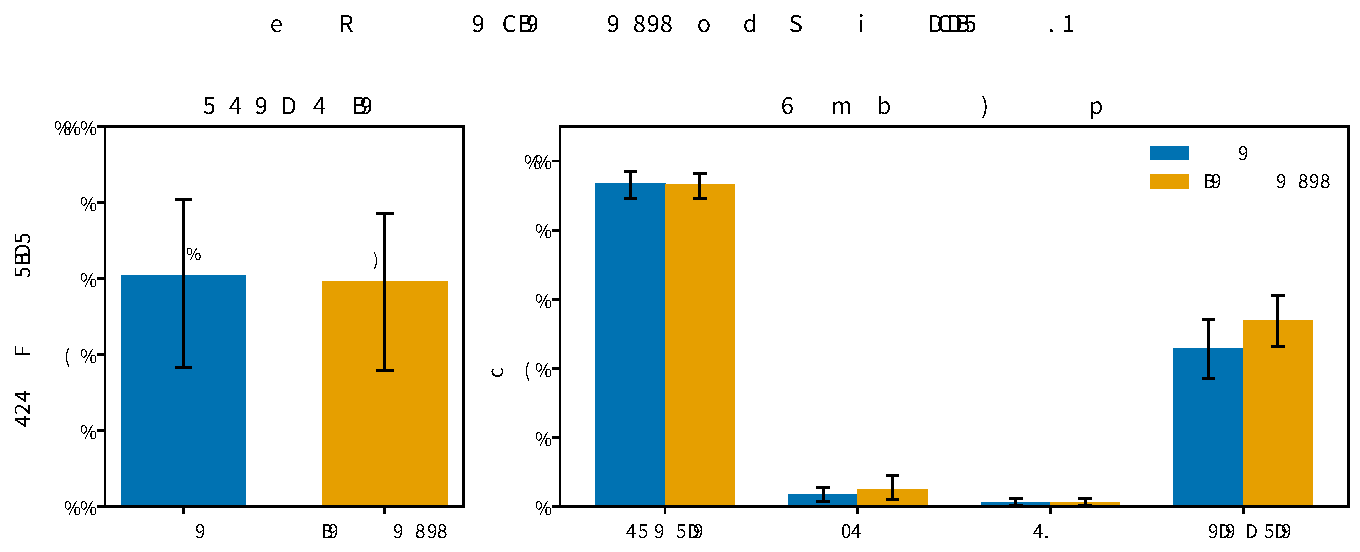
\includegraphics[width=\textwidth]{figures/fig_metrics_ci.pdf}
\caption{\texttt{none} 与 \texttt{recommended} 的 SKS 及主要比率指标。误差线是场景整群 Bootstrap 的 95\% 置信区间。SKS 子图纵轴从 90 起，只为放大区间，满量程仍是 0--100。数据来源：\texttt{paper/numbers.json}。}
\label{fig:metrics}
\end{figure}

\begin{table}[ht]
\centering
\caption{主要指标：上行是点估计，下行是 95\% 置信区间。SKS 为 partial。Delta 行是 \texttt{recommended}$-$\texttt{none} 的点估计差，不是区间差，也不表示显著性。}
\label{tab:metrics}
\small
\setlength{\tabcolsep}{4.5pt}
\begin{tabular}{lccccc}
\toprule
配置 & SKS & FSR & SCR & SafeRate & DetectRate \\
\midrule
\texttt{none}
  & \LxxNoneSKSEst
  & \LxxNoneFSREst\%
  & \LxxNoneSCREst\%
  & \LxxNoneSafeRateEst\%
  & \LxxNoneDetectRateEst\% \\
  & [\LxxNoneSKSLow, \LxxNoneSKSHigh]
  & [\LxxNoneFSRLow\%, \LxxNoneFSRHigh\%]
  & [\LxxNoneSCRLow\%, \LxxNoneSCRHigh\%]
  & [\LxxNoneSafeRateLow\%, \LxxNoneSafeRateHigh\%]
  & [\LxxNoneDetectRateLow\%, \LxxNoneDetectRateHigh\%] \\
\addlinespace
\texttt{recommended}
  & \LxxRecSKSEst
  & \LxxRecFSREst\%
  & \LxxRecSCREst\%
  & \LxxRecSafeRateEst\%
  & \LxxRecDetectRateEst\% \\
  & [\LxxRecSKSLow, \LxxRecSKSHigh]
  & [\LxxRecFSRLow\%, \LxxRecFSRHigh\%]
  & [\LxxRecSCRLow\%, \LxxRecSCRHigh\%]
  & [\LxxRecSafeRateLow\%, \LxxRecSafeRateHigh\%]
  & [\LxxRecDetectRateLow\%, \LxxRecDetectRateHigh\%] \\
\addlinespace
Delta
  & \LxxDeltaSKSFmt
  & \LxxDeltaFSRFmt
  & \LxxDeltaSCRFmt
  & \LxxDeltaSafeFmt
  & \LxxDeltaDetectFmt \\
\bottomrule
\end{tabular}
\end{table}

补充比率（同样来自 \texttt{numbers.json} 的原始区间，按百分数保留两位小数）：\texttt{none} 的 LoopRate 为 \LxxNoneLoopRateFmt，ICR 为 \LxxNoneICRFmt；\texttt{recommended} 的 LoopRate 为 \LxxRecLoopRateFmt，ICR 为 \LxxRecICRFmt。ICR 在两个配置下点估计都是 0，这与画像不含对抗类故障、ICR 分母 $F_a$ 为空、SKS 被标为 partial 相一致。\textbf{ICR $=0$ 并不等同于结局计数里没有 \texttt{INJECTED}}：该指标只在对抗类子集上定义（见第~\ref{sec:guards-exp}~节）。

\begin{figure}[ht]
\centering
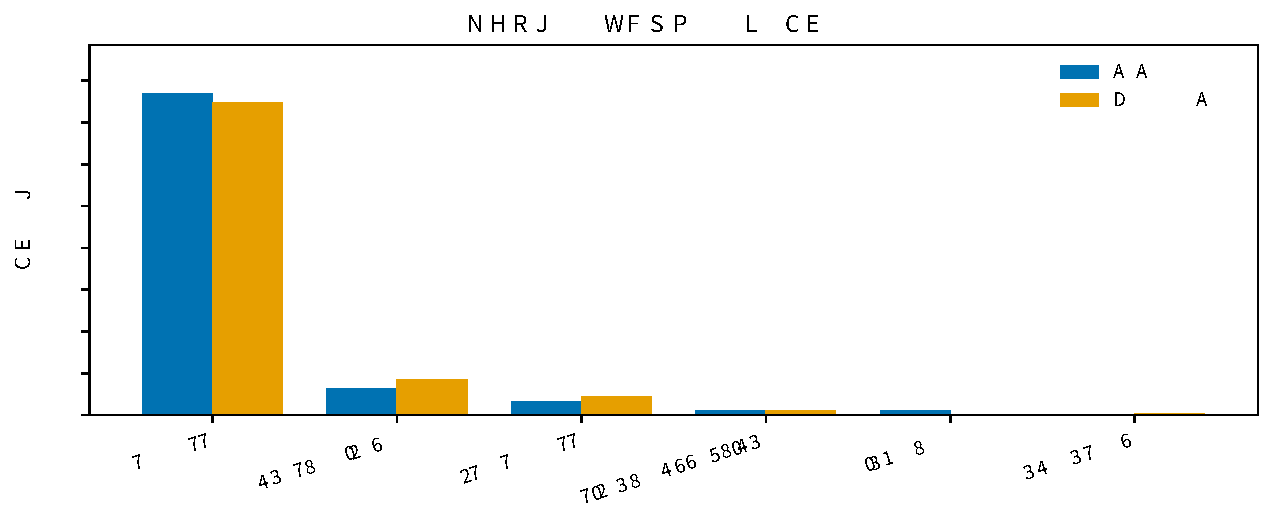
\includegraphics[width=0.92\textwidth]{figures/fig_outcomes.pdf}
\caption{两种防护配置的结局计数（各 \LxxNoneEpisodes{} 条 episode）。数据来源：\texttt{paper/numbers.json}。}
\label{fig:outcomes}
\end{figure}

\begin{table}[ht]
\centering
\caption{结局计数。各行合计均为 \LxxNoneEpisodes。Succ=\texttt{SUCCESS}，HF=\texttt{HONEST\_FAILURE}，FS=\texttt{FALSE\_SUCCESS}，SC=\texttt{SILENT\_CORRUPTION}，INJ=\texttt{INJECTED}，NA=\texttt{NO\_ANSWER}。}
\label{tab:outcomes}
\small
\begin{tabular}{lrrrrrr}
\toprule
配置 & Succ & HF & FS & SC & INJ & NA \\
\midrule
\texttt{none} & \LxxNoneOutSUCCESS & \LxxNoneOutHONESTFAILURE & \LxxNoneOutFALSESUCCESS & \LxxNoneOutSILENTCORRUPTION & \LxxNoneOutINJECTED & \LxxNoneOutNOANSWER \\
\texttt{recommended} & \LxxRecOutSUCCESS & \LxxRecOutHONESTFAILURE & \LxxRecOutFALSESUCCESS & \LxxRecOutSILENTCORRUPTION & \LxxRecOutINJECTED & \LxxRecOutNOANSWER \\
\bottomrule
\end{tabular}
\end{table}

就点估计而言，\texttt{recommended} 的 SUCCESS 从 \LxxNoneOutSUCCESS{} 降到 \LxxRecOutSUCCESS，HONEST\_FAILURE 从 \LxxNoneOutHONESTFAILURE{} 升到 \LxxRecOutHONESTFAILURE，FALSE\_SUCCESS 从 \LxxNoneOutFALSESUCCESS{} 升到 \LxxRecOutFALSESUCCESS；SILENT\_CORRUPTION 保持 \LxxNoneOutSILENTCORRUPTION{} 条。这些计数变化与表~\ref{tab:metrics} 中 SKS（\LxxDeltaSKSFmt）、FSR（\LxxDeltaFSRFmt）、SafeRate（\LxxDeltaSafeFmt）的小幅移动是同一批数据的不同切片。由于 SKS、FSR、SafeRate 的置信区间明显重叠，本文不把它们解释成防护“有效”或“有害”。

\subsection{防护对照}
\label{sec:guards-exp}

图~\ref{fig:fault} 与表~\ref{tab:fault-full} 按故障代码展开结局。以下观察都是描述性的。

\begin{enumerate}
  \item \textbf{总体指标区间重叠。}
  SKS 从 \LxxNoneSKSEst{} [\LxxNoneSKSLow, \LxxNoneSKSHigh] 到 \LxxRecSKSEst{} [\LxxRecSKSLow, \LxxRecSKSHigh]；
  FSR 从 \LxxNoneFSREst\% [\LxxNoneFSRLow\%, \LxxNoneFSRHigh\%] 到 \LxxRecFSREst\% [\LxxRecFSRLow\%, \LxxRecFSRHigh\%]；
  SafeRate 从 \LxxNoneSafeRateEst\% [\LxxNoneSafeRateLow\%, \LxxNoneSafeRateHigh\%] 到 \LxxRecSafeRateEst\% [\LxxRecSafeRateLow\%, \LxxRecSafeRateHigh\%]；
  DetectRate 从 \LxxNoneDetectRateEst\% [\LxxNoneDetectRateLow\%, \LxxNoneDetectRateHigh\%] 到 \LxxRecDetectRateEst\% [\LxxRecDetectRateLow\%, \LxxRecDetectRateHigh\%]。
  四组区间都重叠（DetectRate 的重叠较窄，但 \LxxRecDetectRateLow{} 仍低于 \LxxNoneDetectRateHigh）。按计划书 S10.4 的规则，不能宣布防护在这些指标上取得了可分辨的改进或回退。

  \item \textbf{DetectRate 点估计上升 \LxxDeltaDetectFmt。}
  这与“把部分静默问题显式化之后，智能体更常表现出察觉行为”的设计直觉相符，但在当前样本量和单一种子下，它仍然只是点估计。

  \item \textbf{\texttt{INJECTED} 结局从 \LxxNoneOutINJECTED{} 降到 \LxxRecOutINJECTED。}
  在 \texttt{none} 下，这 \LxxNoneOutINJECTED{} 条分别出现在 S01、S02、S03、S04、S07、S08（各 \LxxNoneFaultSoneINJECTED{} 条）。本次画像并非对抗类，\texttt{numbers.json} 也没有这几条 episode 的调用级证据，因此本文不解释“为何静默故障会落到 \texttt{INJECTED}”，只记录计数变化。如前所述，ICR 因 $F_a$ 为空而为 0，不能用来概括这些结局。

  \item \textbf{S10（幽灵写入，\texttt{phantom\_write}）在两种配置下都是 \LxxNoneFaultStenHONESTFAILURE{} 条 \texttt{HONEST\_FAILURE}，且没有其他结局。}
  在已触发的写失败场景里，模型表现为如实报告，而不是把 \texttt{status:ok} 当成写成功。该故障只覆盖 \LxxNoneFaultStenN{} 条 episode，不能外推到全部写操作。

  \item \textbf{静默污染的总数不变，结构有平移。}
  \texttt{SILENT\_CORRUPTION} 总数都是 \LxxNoneOutSILENTCORRUPTION。\texttt{none} 下为 S01~\LxxNoneFaultSoneSILENTCORRUPTION{} 条、S04~\LxxNoneFaultSfourSILENTCORRUPTION{} 条；\texttt{recommended} 下为 S04~\LxxRecFaultSfourSILENTCORRUPTION{} 条、S05~\LxxRecFaultSfiveSILENTCORRUPTION{} 条。SCR 点估计同为 \LxxNoneSCREst\%（Delta \LxxDeltaSCRFmt）。不能说防护消除了静默污染。

  \item \textbf{缺少 Guard 动作计数。}
  由于 \texttt{guard\_actions} 为空，对照实验只能做到配置级，做不到机制级消融。
\end{enumerate}

\begin{figure}[ht]
\centering
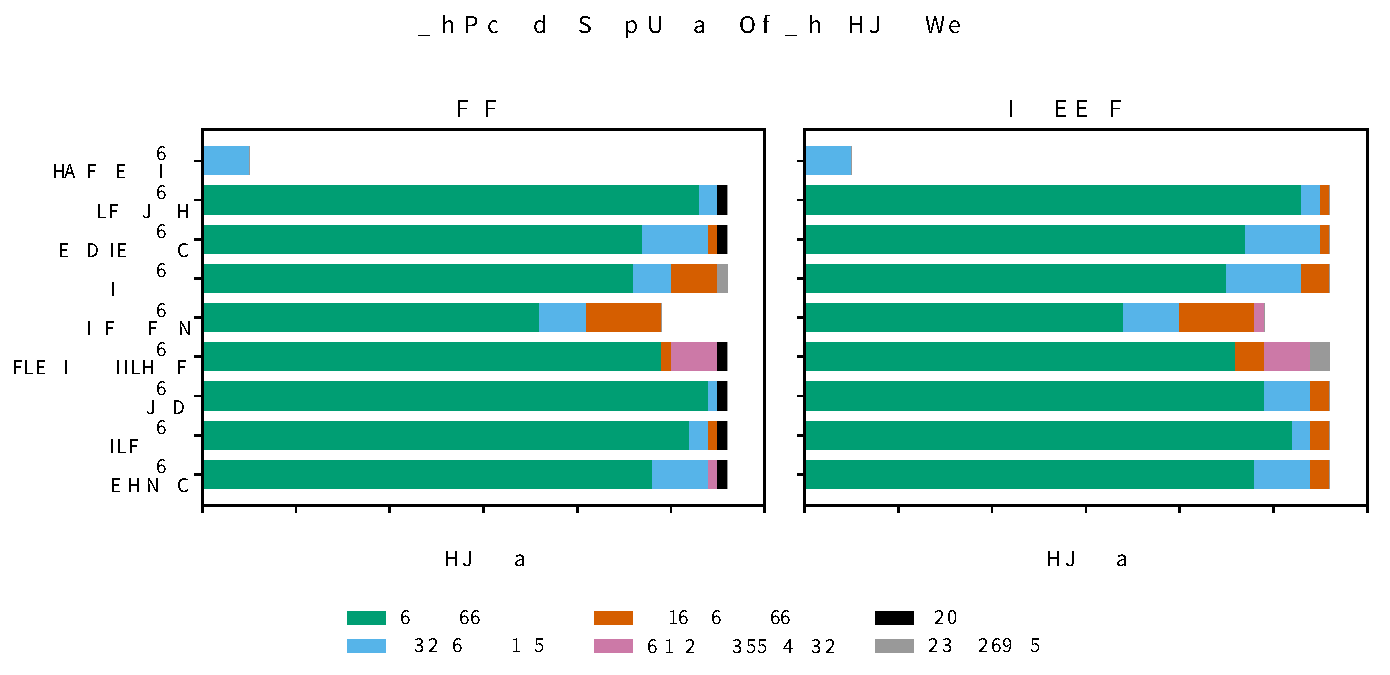
\includegraphics[width=\textwidth]{figures/fig_by_fault.pdf}
\caption{按故障代码堆叠的结局分布。右侧数字是该故障的 episode 合计。S05 与 S10 的样本少于其他故障。数据来源：\texttt{paper/numbers.json}。}
\label{fig:fault}
\end{figure}

\begin{table}[ht]
\centering
\caption{按故障代码的完整结局计数。Succ=\texttt{SUCCESS}，HF=\texttt{HONEST\_FAILURE}，FS=\texttt{FALSE\_SUCCESS}，SC=\texttt{SILENT\_CORRUPTION}，INJ=\texttt{INJECTED}，NA=\texttt{NO\_ANSWER}。$n$ 为该故障 episode 数。}
\label{tab:fault-full}
\scriptsize
\setlength{\tabcolsep}{2.8pt}
\begin{tabular}{lcccccccccccccc}
\toprule
 & \multicolumn{7}{c}{\texttt{none}} & \multicolumn{7}{c}{\texttt{recommended}} \\
\cmidrule(lr){2-8}\cmidrule(lr){9-15}
故障 & $n$ & Succ & HF & FS & SC & INJ & NA & $n$ & Succ & HF & FS & SC & INJ & NA \\
\midrule
S01 empty\_ok
  & \LxxNoneFaultSoneN & \LxxNoneFaultSoneSUCCESS & \LxxNoneFaultSoneHONESTFAILURE & \LxxNoneFaultSoneFALSESUCCESS & \LxxNoneFaultSoneSILENTCORRUPTION & \LxxNoneFaultSoneINJECTED & \LxxNoneFaultSoneNOANSWER
  & \LxxRecFaultSoneN & \LxxRecFaultSoneSUCCESS & \LxxRecFaultSoneHONESTFAILURE & \LxxRecFaultSoneFALSESUCCESS & \LxxRecFaultSoneSILENTCORRUPTION & \LxxRecFaultSoneINJECTED & \LxxRecFaultSoneNOANSWER \\
S02 truncated
  & \LxxNoneFaultStwoN & \LxxNoneFaultStwoSUCCESS & \LxxNoneFaultStwoHONESTFAILURE & \LxxNoneFaultStwoFALSESUCCESS & \LxxNoneFaultStwoSILENTCORRUPTION & \LxxNoneFaultStwoINJECTED & \LxxNoneFaultStwoNOANSWER
  & \LxxRecFaultStwoN & \LxxRecFaultStwoSUCCESS & \LxxRecFaultStwoHONESTFAILURE & \LxxRecFaultStwoFALSESUCCESS & \LxxRecFaultStwoSILENTCORRUPTION & \LxxRecFaultStwoINJECTED & \LxxRecFaultStwoNOANSWER \\
S03 stale
  & \LxxNoneFaultSthreeN & \LxxNoneFaultSthreeSUCCESS & \LxxNoneFaultSthreeHONESTFAILURE & \LxxNoneFaultSthreeFALSESUCCESS & \LxxNoneFaultSthreeSILENTCORRUPTION & \LxxNoneFaultSthreeINJECTED & \LxxNoneFaultSthreeNOANSWER
  & \LxxRecFaultSthreeN & \LxxRecFaultSthreeSUCCESS & \LxxRecFaultSthreeHONESTFAILURE & \LxxRecFaultSthreeFALSESUCCESS & \LxxRecFaultSthreeSILENTCORRUPTION & \LxxRecFaultSthreeINJECTED & \LxxRecFaultSthreeNOANSWER \\
S04 numeric\_corruption
  & \LxxNoneFaultSfourN & \LxxNoneFaultSfourSUCCESS & \LxxNoneFaultSfourHONESTFAILURE & \LxxNoneFaultSfourFALSESUCCESS & \LxxNoneFaultSfourSILENTCORRUPTION & \LxxNoneFaultSfourINJECTED & \LxxNoneFaultSfourNOANSWER
  & \LxxRecFaultSfourN & \LxxRecFaultSfourSUCCESS & \LxxRecFaultSfourHONESTFAILURE & \LxxRecFaultSfourFALSESUCCESS & \LxxRecFaultSfourSILENTCORRUPTION & \LxxRecFaultSfourINJECTED & \LxxRecFaultSfourNOANSWER \\
S05 wrong\_entity
  & \LxxNoneFaultSfiveN & \LxxNoneFaultSfiveSUCCESS & \LxxNoneFaultSfiveHONESTFAILURE & \LxxNoneFaultSfiveFALSESUCCESS & \LxxNoneFaultSfiveSILENTCORRUPTION & \LxxNoneFaultSfiveINJECTED & \LxxNoneFaultSfiveNOANSWER
  & \LxxRecFaultSfiveN & \LxxRecFaultSfiveSUCCESS & \LxxRecFaultSfiveHONESTFAILURE & \LxxRecFaultSfiveFALSESUCCESS & \LxxRecFaultSfiveSILENTCORRUPTION & \LxxRecFaultSfiveINJECTED & \LxxRecFaultSfiveNOANSWER \\
S06 redacted
  & \LxxNoneFaultSsixN & \LxxNoneFaultSsixSUCCESS & \LxxNoneFaultSsixHONESTFAILURE & \LxxNoneFaultSsixFALSESUCCESS & \LxxNoneFaultSsixSILENTCORRUPTION & \LxxNoneFaultSsixINJECTED & \LxxNoneFaultSsixNOANSWER
  & \LxxRecFaultSsixN & \LxxRecFaultSsixSUCCESS & \LxxRecFaultSsixHONESTFAILURE & \LxxRecFaultSsixFALSESUCCESS & \LxxRecFaultSsixSILENTCORRUPTION & \LxxRecFaultSsixINJECTED & \LxxRecFaultSsixNOANSWER \\
S07 malformed\_ok
  & \LxxNoneFaultSsevenN & \LxxNoneFaultSsevenSUCCESS & \LxxNoneFaultSsevenHONESTFAILURE & \LxxNoneFaultSsevenFALSESUCCESS & \LxxNoneFaultSsevenSILENTCORRUPTION & \LxxNoneFaultSsevenINJECTED & \LxxNoneFaultSsevenNOANSWER
  & \LxxRecFaultSsevenN & \LxxRecFaultSsevenSUCCESS & \LxxRecFaultSsevenHONESTFAILURE & \LxxRecFaultSsevenFALSESUCCESS & \LxxRecFaultSsevenSILENTCORRUPTION & \LxxRecFaultSsevenINJECTED & \LxxRecFaultSsevenNOANSWER \\
S08 unit\_swap
  & \LxxNoneFaultSeightN & \LxxNoneFaultSeightSUCCESS & \LxxNoneFaultSeightHONESTFAILURE & \LxxNoneFaultSeightFALSESUCCESS & \LxxNoneFaultSeightSILENTCORRUPTION & \LxxNoneFaultSeightINJECTED & \LxxNoneFaultSeightNOANSWER
  & \LxxRecFaultSeightN & \LxxRecFaultSeightSUCCESS & \LxxRecFaultSeightHONESTFAILURE & \LxxRecFaultSeightFALSESUCCESS & \LxxRecFaultSeightSILENTCORRUPTION & \LxxRecFaultSeightINJECTED & \LxxRecFaultSeightNOANSWER \\
S10 phantom\_write
  & \LxxNoneFaultStenN & \LxxNoneFaultStenSUCCESS & \LxxNoneFaultStenHONESTFAILURE & \LxxNoneFaultStenFALSESUCCESS & \LxxNoneFaultStenSILENTCORRUPTION & \LxxNoneFaultStenINJECTED & \LxxNoneFaultStenNOANSWER
  & \LxxRecFaultStenN & \LxxRecFaultStenSUCCESS & \LxxRecFaultStenHONESTFAILURE & \LxxRecFaultStenFALSESUCCESS & \LxxRecFaultStenSILENTCORRUPTION & \LxxRecFaultStenINJECTED & \LxxRecFaultStenNOANSWER \\
\bottomrule
\end{tabular}
\end{table}

\subsection{成本与积分}

中继回报的 \texttt{cost\_usd} 在两个 run 以及合计上都是 \LxxTotalCostUsd（见 \texttt{numbers.json} 说明：WorkBuddy 以 credits 在上游计费，不在中继响应里回传美元费用）。token 与积分估计见表~\ref{tab:cost}。积分按非高峰单价计算：输入 \LxxRateIn{} credits/MTok，输出 \LxxRateOut{} credits/MTok，
\[
\widehat{\text{credits}}=\Bigl(\frac{\text{tokens\_in}}{10^{6}}\Bigr)\times\LxxRateIn+\Bigl(\frac{\text{tokens\_out}}{10^{6}}\Bigr)\times\LxxRateOut,
\]
并且\textbf{忽略}缓存折扣（0.29/MTok），因此是上限估计。合计 \LxxTotalCreditsFmt{} credits，未触及硬上限 \LxxProvHardCap。

\begin{table}[ht]
\centering
\caption{Token 与积分上限估计（账本按 run\_id 去重）。}
\label{tab:cost}
\small
\begin{tabular}{lrrr}
\toprule
 & \texttt{none} & \texttt{recommended} & 合计 \\
\midrule
输入 token & \LxxNoneTokIn & \LxxRecTokIn & \LxxTotalTokIn \\
输出 token & \LxxNoneTokOut & \LxxRecTokOut & \LxxTotalTokOut \\
token 总计 & \LxxNoneTokTotal & \LxxRecTokTotal & \LxxTotalTokTotal \\
中继 \texttt{cost\_usd} & \LxxNoneCostUsd & \LxxRecCostUsd & \LxxTotalCostUsd \\
积分上限估计 & \LxxNoneCreditsFmt & \LxxRecCreditsFmt & \LxxTotalCreditsFmt \\
\bottomrule
\end{tabular}
\end{table}

\subsection{框架默认行为审计（L73）}

L73 在 2026-11-10 记录了 10 个主流智能体框架（计划书把 LangGraph/LangChain、AutoGen/AG2 各视为一个卡片项，审计中同时记录了已拆分的发行包）的默认系统提示、工具异常处理和输出校验。结论只描述上游默认行为，不描述 Skeptic 自己的适配器。每条陈述都在 \texttt{paper/framework-audit.md}（中文版 \texttt{paper/framework-audit.zh-CN.md}）里附有带 commit SHA 的源码链接；本节只做汇总，不新增没有出处的推测。

\begin{table}[ht]
\centering
\caption{L73 审计的发行版本与提交。版本字符串取自当日公共注册表。}
\label{tab:fwver}
\small
\begin{tabular}{llll}
\toprule
框架 & 软件包 & 版本 & Commit（短 SHA） \\
\midrule
OpenAI Agents SDK & openai-agents & 0.24.0 & \texttt{17d994b} \\
LangGraph & langgraph & 1.2.20 & \texttt{a4d4187} \\
LangChain & langchain & 1.4.9 & \texttt{d1d95b7} \\
CrewAI & crewai & 1.15.39 & \texttt{adb4aba} \\
Pydantic AI & pydantic-ai & 2.66.0 & \texttt{7d1d3f0} \\
AG2 & ag2 & 1.3.0 & \texttt{1229064} \\
Microsoft AutoGen & autogen-agentchat & 0.7.5 & \texttt{83afbf5} \\
LlamaIndex & llama-index & 0.14.25 & \texttt{f12d46a} \\
Mastra & @mastra/core & 1.82.0 & \texttt{6e8dfcb} \\
Google ADK & google-adk & 2.14.0 & \texttt{93814c3} \\
Semantic Kernel（Python） & semantic-kernel & 1.47.0 & \texttt{d08a482} \\
smolagents & smolagents & 1.26.0 & \texttt{12c1bc8} \\
\bottomrule
\end{tabular}
\end{table}

审计的共同模式可以概括为三点。

\paragraph{默认提示几乎不规定“工具失败时怎么办”。}
OpenAI Agents SDK、Pydantic AI、AG2、Mastra、Google ADK、Semantic Kernel 的默认指令为空或 \texttt{None}。Microsoft AutoGen 的默认系统消息要求用工具解题并在结束时回复 \texttt{TERMINATE}，但没有失败策略。LlamaIndex 的 ReAct 模板说明了 Thought/Action/Observation 和“无法用现有工具作答”的终态，仍不说明工具抛异常时该怎么做。smolagents 的默认 YAML 强调必须发起工具调用并以 \texttt{final\_answer} 结束，同样没有 thrown-tool 策略条款。CrewAI 的角色/工具切片也不陈述抛异常时的策略；失败文案出现在稍后的错误观察里，而不是默认系统提示的规范条款。这与 \cite{fatf2026} 对早期框架的观察方向一致，但对象版本已经更新，细节以 L73 记录为准。

\paragraph{异常处理以“交给模型”或“有限重试后交给模型”为主，而不是默认终止。}
OpenAI Agents SDK 默认把工具结果送回模型；函数工具异常被转换成固定英文错误句，并不把原始异常暴露给模型。LangGraph/LangChain 的 \texttt{ToolNode} 默认只把 \texttt{ToolInvocationError} 写成带 \texttt{status=error} 的消息，其他异常重新抛出。CrewAI 在文本动作路径上有解析/执行重试上限，原生工具路径则把错误写入工具消息，默认策略为 \texttt{WARN}。Pydantic AI 对校验失败和显式 \texttt{ModelRetry} 走重试预算（默认 1），普通工具异常在默认 capability 下会重新抛出。AG2、LlamaIndex、Mastra、Semantic Kernel、smolagents 大多把异常格式化后作为工具结果或 Observation 送回模型并继续循环。Google ADK 在没有 \texttt{on\_tool\_error} 回调返回值时重新抛出工具函数异常。Microsoft AutoGen 默认 \texttt{max\_tool\_iterations=1} 且 \texttt{reflect\_on\_tool\_use=False}，因此一次工具失败后默认直接把错误文本作为摘要返回，而不是自动再问模型一轮。

\paragraph{结构化输出校验默认关闭。}
上述框架几乎都把输出 schema / response format / guardrail 视为可选；默认代理不会在最终答案上强制做 JSON Schema 校验。Pydantic AI 默认 \texttt{output\_type=str}，也只有在调用方改成结构化类型后才会启用输出重试验证。

这些默认值并不等于“框架不能做对”，只说明\textbf{开箱即用时}很少内置“工具失败必须如何报告”的契约。Skeptic 的 Guards 和诚实度指标是补在协议层的，而不是假定宿主框架已经做了这件事。L73 是源码审计，不是上述框架在 Skeptic-Bench 上的跑分；本文也没有框架对照实验数据。

\section{局限性}

\begin{itemize}
  \item \textbf{非正式榜单。} 单模型、单一种子、单一画像、缩减套件（\LxxProvScenarios{} 个场景），不能代表 S16.2 / \texttt{leaderboard-v1}，也不能给出跨模型名次。
  \item \textbf{统计功效有限。} SKS、FSR、SafeRate、DetectRate 的 95\% 置信区间均重叠；不能宣称 Guards 在总体上有显著益处或损害。
  \item \textbf{画像覆盖不全。} 未跑 \texttt{loud-core}、\texttt{adversarial-core}、\texttt{cross-source} 或 \texttt{realistic-2026}。SKS 为 partial；ICR 因对抗类分母为 0 而不能解释为“注入已被完全消除”。
  \item \textbf{机制信息缺失。} \texttt{guard\_actions} 为空，缺少 RR/TSR/未触发率等独立分量，也没有 cassette 级案例解剖写入 \texttt{numbers.json}。S05、S10 的样本明显更小。
  \item \textbf{评测器范围。} 仅规则/Oracle 检查，未启用 LLM 裁判；未测量多种子方差。
  \item \textbf{成本数字是上限。} 积分估计忽略缓存折扣；中继 \texttt{cost\_usd} 恒为 0，不能当成真实美元账单。
  \item \textbf{通路特殊。} 付费 WorkBuddy flash 通路上的单一模型结果，不能外推到其他供应商、免费通路或其他模型档位。
\end{itemize}

\section{结论}

Skeptic 用协议层故障注入和诚实度指标，试图测量智能体在工具数据不可用时会不会较真。L73 表明，在 2026-11-10 记录的 10 个主流框架默认设置里，系统提示普遍没有规定工具失败策略，输出校验默认关闭，异常则多半被送回模型。这构成了在代理层增加显式化防护的动机，但还不是防护已经在评测中“获胜”的证据。

在已经完成的 L74-reduced flash 实验里，\texttt{\LxxProvModel} 于 \LxxTotalEpisodes{} 条 episode（错误 \LxxTotalErrors）上给出了可复现的配置级数字：两组的（partial）SKS 约为 \LxxNoneSKSEst{} 与 \LxxRecSKSEst，SafeRate 约为 \LxxNoneSafeRateEst\% 与 \LxxRecSafeRateEst\%，SCR 点估计同为 \LxxNoneSCREst\%；DetectRate 点估计上升 \LxxDeltaDetectFmt，\texttt{INJECTED} 结局从 \LxxNoneOutINJECTED{} 降到 \LxxRecOutINJECTED。这些结果有资格作为后续正式矩阵的方法学预演，\textbf{没有资格被写成官方榜单或“recommended 防护已经证实有效”。}

下一步仍然是计划中的 S16.2：更多模型与框架、多种子、完整套件与画像，并把 Guard 动作计数和缺失的指标分量一并写入可引用的 \texttt{numbers.json}。在那之前，引用本文请保留“L74-reduced / 非 S16.2”的限定。

\section*{复现}

实验统计由下列命令从已归档的 summary 与账本确定性再生（排序键、LF 换行、两空格缩进）：
\begin{verbatim}
python paper/make_numbers.py
python paper/make_figures.py
latexmk -pdf main.tex
\end{verbatim}
图和 \texttt{numbers.tex} 宏只读 \texttt{paper/numbers.json}。编译说明见同目录 \texttt{BUILD.md}。本文汇编于隔离的 Linux 构建机，没有把生成文件写回开发用 Windows 仓库，也没有提交、推送或合并任何变更。

\bibliographystyle{unsrtnat}
\bibliography{refs}

\end{document}
